\documentclass[12pt]{article}
	
\usepackage[margin=1in]{geometry}		% For setting margins
\usepackage{amsmath}				% For Math
\usepackage{amssymb} % For \mathbb
\usepackage{fancyhdr}				% For fancy header/footer
\usepackage{graphicx}	% For including figure/image
\renewcommand{\contentsname}{Table of Contents}
\usepackage{enumitem}
\usepackage{cancel}					% To use the slash to cancel out stuff in work
\usepackage[margin=0.25in]{geometry}
\usepackage{hyperref}
\usepackage{float}
\usepackage{indentfirst}
\usepackage[american, siunitx]{circuitikz}
\usepackage{circuitikz}
\usepackage{lipsum}
\usepackage{setspace}
\usepackage{tikz, tcolorbox} 
\usepackage[dvipsnames]{xcolor}
\usepackage{fontspec}
\setmainfont{Times New Roman}



\pagestyle{fancy}
\fancyhead[LO,L]{Mark Le} % replace with your name!
\fancyhead[CO,C]{}
\fancyhead[RO,R]{\textbf{ELECENG 2EI4 Project 4 - CMOS XOR Gate}}
\fancyfoot[LO,L]{}
\fancyfoot[CO,C]{\textbf{\thepage}}
\fancyfoot[RO,R]{}


%%%%%%%%%%%%%%%%%%%%%%

\spacing{1.25}
\begin{document}
    
    \begin{titlepage}
    \begin{center}
    \vspace*{\fill}

    {\LARGE \textbf{ELECENG 2EI4 - Electronic Devices \& Circuits I}\par}
    \vspace{2.5cm}

    {\LARGE\bfseries Project 4 - CMOS XOR Gate\par}
    \vspace{2.5cm}
    
    {\Large \textbf{Mark Le - 400558145}\par}
    \vspace{2.5cm}
    
    {\large \textbf{Instructor:} Dr. Yaser M. Haddara\par}
    \vspace{0.5cm}
    {\large \textbf{Term:} Winter 2026 \par}
    \vspace{0.5cm}
    
    {\large \textbf{Submission Deadline:} Sunday, April 5, 2026\par}
    \end{center}

    \vspace*{\fill}

    \textbf{Statement of Originality:} As a future member of the engineering profession, the student is responsible for performing the required work in an honest manner, without plagiarism and cheating. Submitting this work with my name and student number is a statement and understanding that this work is my own and adheres to the Academic Integrity Policy of McMaster University and the Code of Conduct of the Professional Engineers of Ontario. Submitted by \textbf{Mark Le, lek37, 400558145}

\end{titlepage}

    \newpage
    \tableofcontents


    \newpage

    \section{Circuit Schematics \& Sizing}

    \subsection{Circuit Schematics}

    For an XOR gate \(Y=A \oplus B\), we can derive the Boolean function in terms of AND, OR, and NOT operations:

    Truth table:

    \vspace{0.3cm}
    \begin{tabular}{|c|c|c|}
    \hline
        A & B & Y \\ \hline
        0 & 0 & 0 \\ \hline 
        0 & 1 & 1 \\ \hline
        1 & 0 & 1 \\ \hline
        1 & 1 & 0 \\ \hline
    \end{tabular}

    Next, we can derive the Boolean expression to be able to implement the CMOS gate easier, using knowledge from \textbf{COMPENG 2DI4 - Logic Design} course

    \[Y=A \oplus B\]
    \[Y=A'B+AB'\hspace{2cm} \text{equivalency}\]
    \[Y=[(A'B+AB')']' \hspace{2cm} \text{double inversion}\]
    \[Y=[(A'B)'(AB')']' \hspace{2cm} \text{DeMorgan's Theorem}\]
    \[Y=[(A+B')(A'+B)]' \hspace{2cm} \text{DeMorgan's Theorem}\]
    \[Y=(AA'+AB+A'B'+BB')' \hspace{2cm} \text{expanding}\]
    \[\boxed{Y=(AB+A'B')'}\]
    \newpage
    CMOS circuit schematics:

    
    \begin{tabular}{cc}
       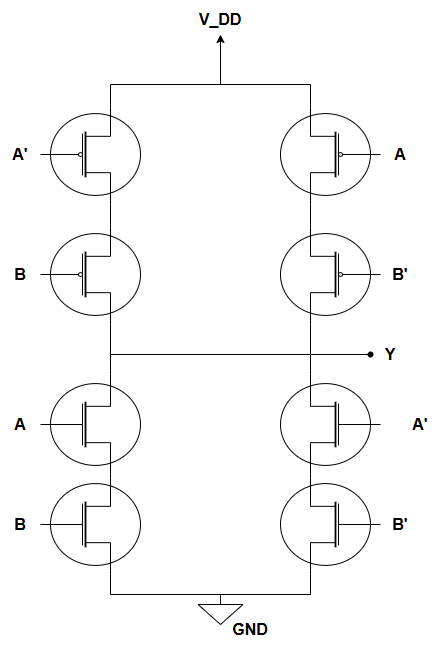
\includegraphics[width=0.4\linewidth]{Screenshot 2026-04-05 035108.png}  & 
       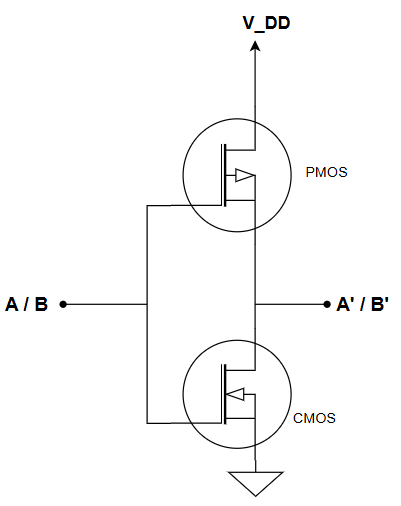
\includegraphics[width=0.4\linewidth]{Screenshot 2026-04-05 120321.png}\\
       XOR CMOS schematics   & CMOS Inverter \\ 
    \end{tabular}


    \subsection{Ideal Sizing}

    For this CMOS network, it can be seen that the pull-up network (PUN) and the pull-down network (PDN) are symmetrical. Therefore, the design must ensures that both networks have equal propagation delays, and minimizing the total delays of the whole network. It is known that the electron mobility of the NMOS is almost 2.5 times larger than PMOS, means that NMOS conducts 2.5 betters than PMOS. To compensate for the worse conducting performance of the PMOS, PMOS must be sized larger than NMOS. Thus, this results in \((W/L)_p=5\) and \((W/L)_n=2\).


    Also from the CMOS-based XOR network above, the longest path for both PDN and PUN network involves two transistors in series. Therefore, the total network \(R_{eq}\) for each network is halved, which leads to \(n/2\) for PDN and \(p/2\) for PUN.  


    As discussed, this design must ensures equal propagation delays for both PUN and PDN network, therefore:
    \[\frac{2P}{2N}=\frac{5}{2}=2.5 \Rightarrow \frac{P}{N}=2.5\]

    So the size of the PMOS must be approximately 2.5 times larger than NMOS size in order to acheive minimum propagation delay. 


    \subsection{Ideal Sizing Feasibility}

    In the scope of this course, the ideal sizing is unfortunately couldn't guaranteed. This is because the NMOS and the PMOS in the kit has fixed value of width and length provided by the manufacturer, and therefore it is expected that the minimum propagation delay may or may not achieved in the timing analysis section below. 
    
  
    \section{Testing on AD3}

    Circuit built on breadboard:

    \begin{center}
        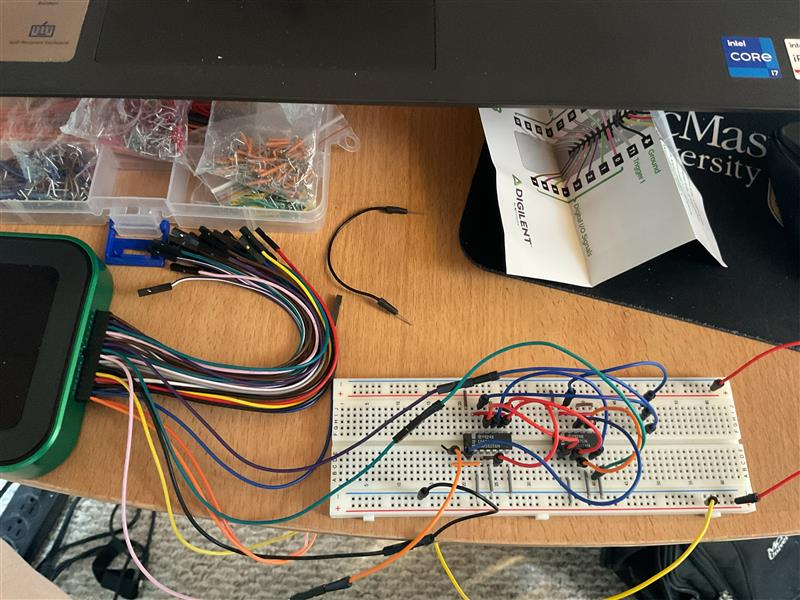
\includegraphics[width=0.7\linewidth]{Image (4).jpg}
    \end{center}


    \subsection{Functional Testing}

    For this circuit, DIO 0 probe of the AD3 is connected to input A of the XOR gate, DIO 1 probe of the AD3 is connected to input B of the AD3, and DIO 2 probe is connected to the output Y. Then, \(V_{DD}\) is supplied by Wavegen W1 at 5V DC. 


    Then, the \textbf{Pattern 1} channel is configure as the following. The goal is to test the circuit with all four possible digital input combinations. Refer to the figure below 
    \begin{itemize}
        \item DIO 0 - Input A is configured as a clock signal at 2 kHz
        \item DIO 1 - Input B is configured as a clock signal at 1 kHz
    \end{itemize}

    \begin{center}
        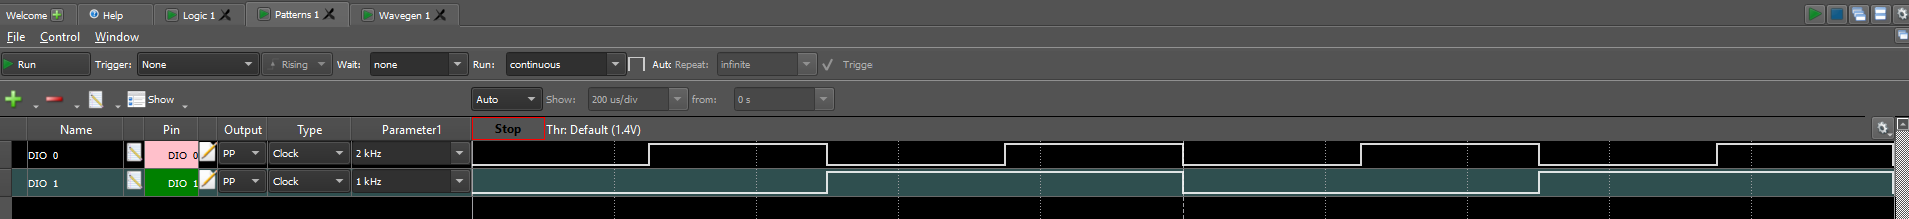
\includegraphics[width=1.0\linewidth]{Screenshot 2026-04-05 154104.png}
    \end{center}

    Finally, running the \textbf{Logic 1} channel produce the following output. It can be seen that the output is exactly what is expected for an XOR gate: 

    \begin{center}
        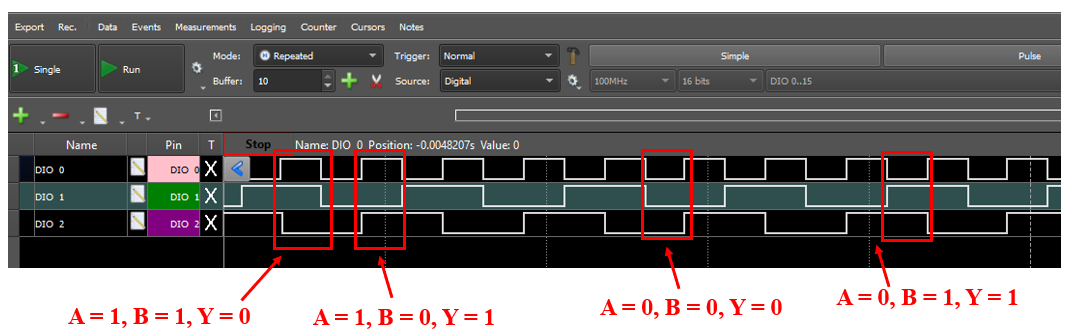
\includegraphics[width=0.9\linewidth]{Screenshot 2026-04-05 155931.png}
    \end{center}

   
    \subsection{Static Level Testing}

    The measurement result on the below figure uses input A as the square wave from 0 - 5V, and input B is the 5V DC supply. Channel 1+ is placed at input A, 1- at GND, 2+ at output Y, 2- at GND. 

    \begin{center}
        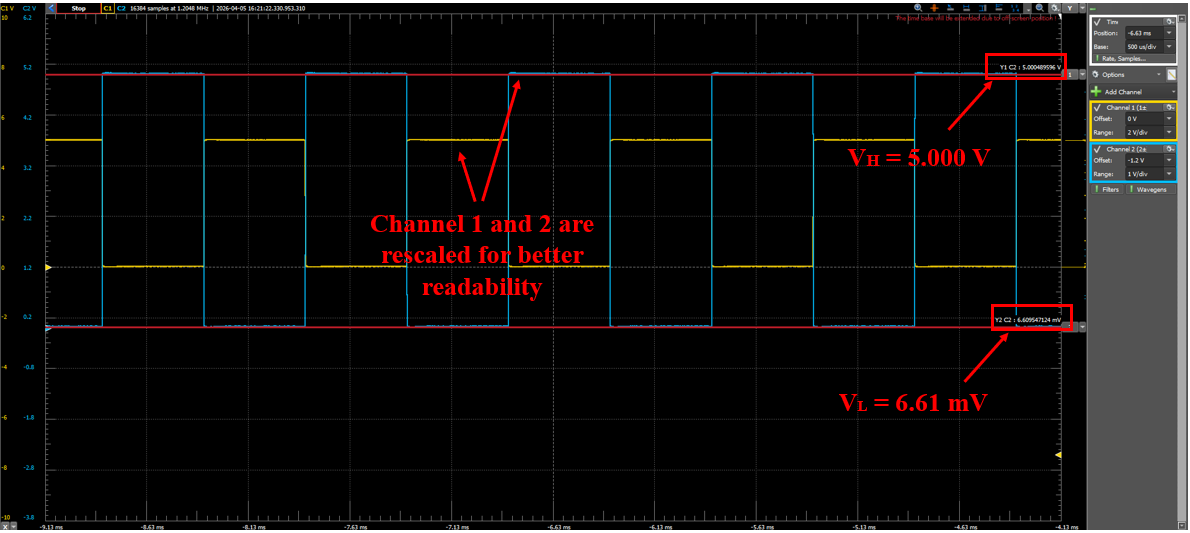
\includegraphics[width=0.9\linewidth]{Screenshot 2026-04-05 162604.png}
    \end{center}


    It can be seen that \(V_H=5.000V\) and \(V_L=6.61mV\), which is expected as the standard voltage for both HIGH and LOW logic. 


    The measurement result on the below figure uses input B as the square wave from 0 to 5V, and input B is the 5V DC supply. 

    \begin{center}
        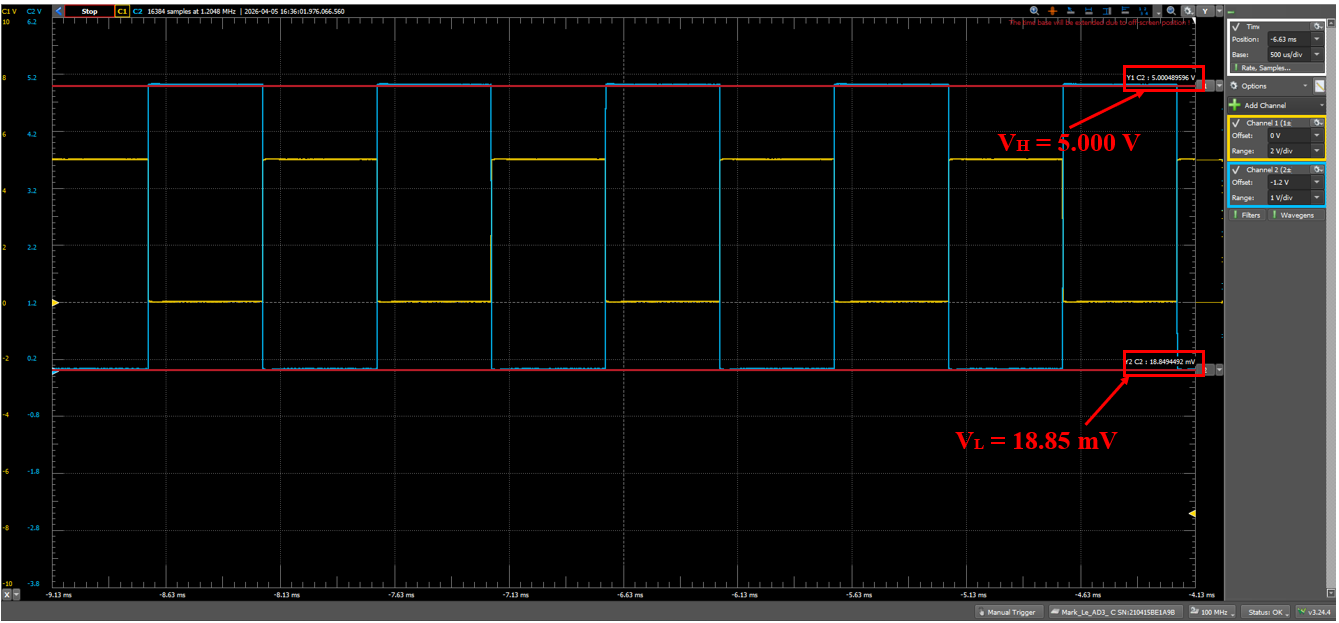
\includegraphics[width=0.9\linewidth]{Screenshot 2026-04-05 163902.png}
    \end{center}

    Also, it can be see that \(V_H=5.000 V\) and \(V_L=18.85mV\). The value of \(V_L\) is a bit higher than \(V_L\) before, but it is still in the normal range for a standard voltage at logic LOW and the impact of switching input probes can be easily negligible. 


    \newpage
    \section{Timing Analysis}

    \subsection{Rise \& Fall Time}
    \begin{center}
        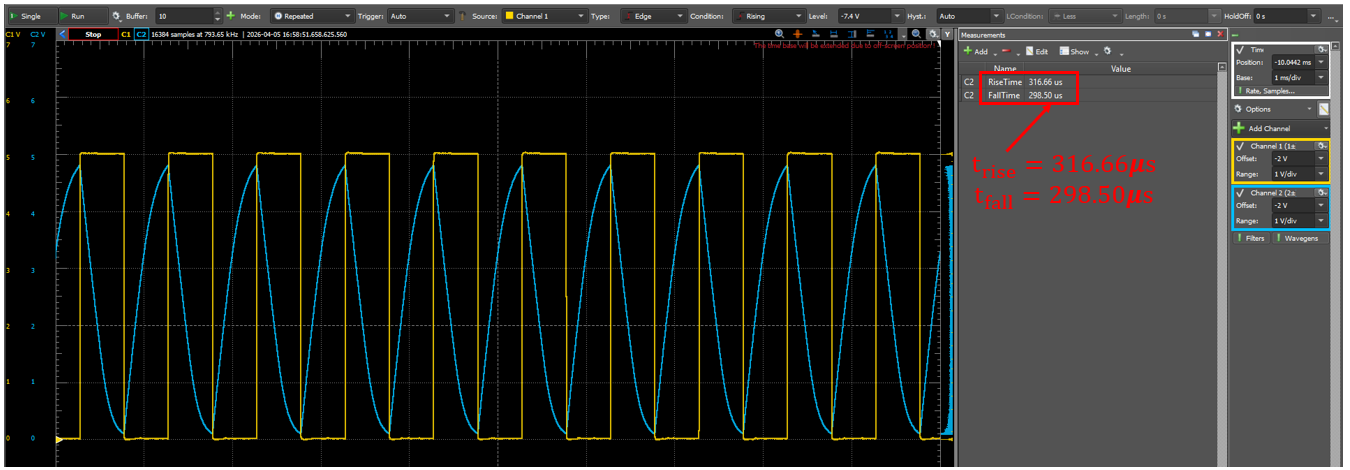
\includegraphics[width=1.0\linewidth]{Screenshot 2026-04-05 170332.png}
    \end{center}

    As it can be seen from the plot of voltage at output \(Y\), the rise time is found to be \(316.66\mu s\), and the fall time is found to be \(298.50\mu s\). 



    \subsection{Experimental Result Of \(\tau_{pHL}, \tau_{pLH}, \tau_p\)}

    To find the value of low-to-high propagation delay \(\tau_{pLH}\), two cursors are needed: one at the point where input (yellow) falls to 50\% of the value range(0 - 5V, 50\% corresponds to 2.5 V), and one at the moment where the output rises to 50\% of the voltage range (0.1 V - 4.8V, 50\% corresponding to 2.45 V), and measure the horizontal difference between the two cursor. AD3 measurement on the plot below shows that \(\boxed{\tau_{pLH}=160.24\mu s}\). 

    \begin{center}
        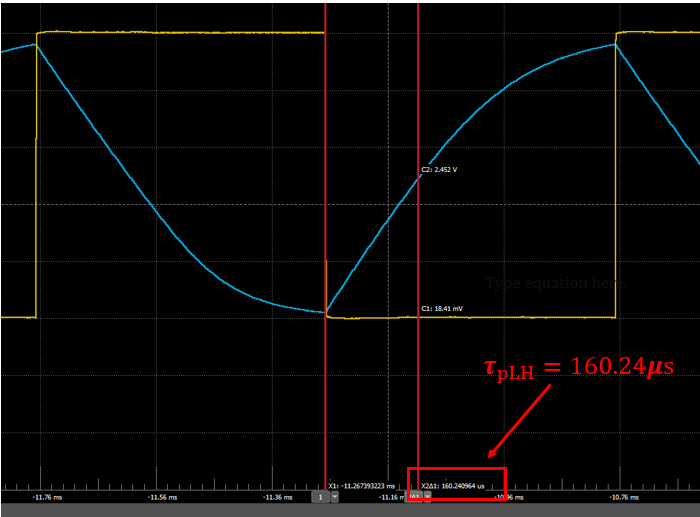
\includegraphics[width=0.6\linewidth]{Screenshot 2026-04-05 175351.png}
    \end{center}

    \newpage
    To find the value of high-to-low propagation delay \(\tau_{pHL}\), two cursors are needed: one at the point where input (yellow) rises to 50\% of the value range (0 to 5V, 50\% corresponds to 2.5 V), and one at the moment where the output falls to 50\% of the voltage range (0.1 V - 4.8V, 50\% corresponding to 2.45 V), and measure the horizontal difference between the two cursor. AD3 measurement on the plot below shows that \(\boxed{\tau_{pHL}=164.31\mu s}\). 

    \begin{center}
        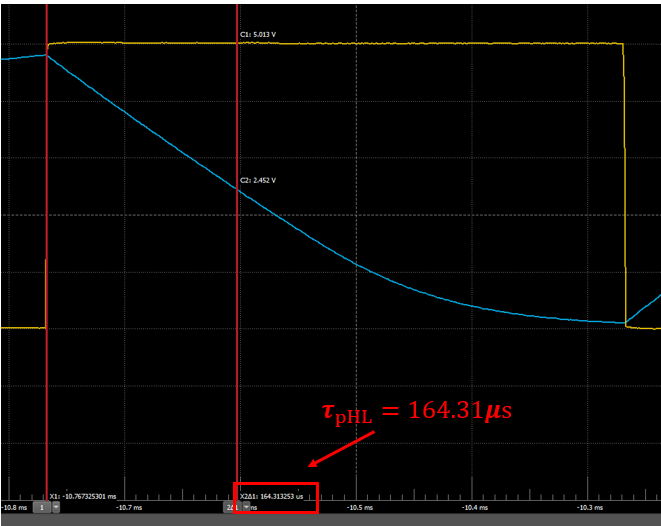
\includegraphics[width=0.7\linewidth]{Screenshot 2026-04-05 180250.png}
    \end{center}

    Finally, once \(\tau_{pHL}\) and \(\tau_{pLH}\) are obtained, the overall propagation delay \(\tau_p\) is calculated by taking the mean of two those values:

    \[\tau_p=\frac{\tau_{pLH}+\tau_{pHL}}{2}=\frac{160.24\mu s+164.31\mu s}{2}=\boxed{162.28 \mu s}\]
    
\end{document}